\chapter{Realisierung}
\label{ref:realisierung}
Dieses Kapitel widmet sich der Realisierung der Applikation inklusive der grafischen Erscheinung. Zudem werden die wichtigsten Infos, um einem Entwickler beim Industriepartner einen schnellen Einstieg in das Weiterführen des Projektes zu ermöglichen, vermittelt.


\section{Aktuelle Erscheinung}
\textbf{Activity}

Die \textit{RadioTour} App besteht aus einer Activity wie in Abbildung \ref{gesamteactivity} dargestellt wird. Diese Activity wird in zwei Hauptteile eingeteilt. Es sind dies der (1)Header- sowie der (2)Hauptbereich. 

Activity:
\begin{lstlisting}{Name}
package ch.hsr.sa.radiotour.activities;
public class RadioTourActivity extends Activity 
	implements Observer, OnClickListener
\end{lstlisting}


View definiert in:
\textit{res/layout/base\_activity.xml}

Die \textit{RadioTourActivity} Klasse ist der Startpunkt der Applikationsausführung und deshalb im \textit{AndroidManifest.xml} File als Startactivity eingetragen. Das AndroiManifest.xml ist eine Datei welche in jedem Android Projekt im Stammverzeichnis vorhanden sein muss. Es enthält wichtige Informationen zur Applikation, unter anderem die Startactivity.


\begin{figure}[h!]
\caption{Gesamte Activity}
\label{fig:gesamteactivity}
\centering
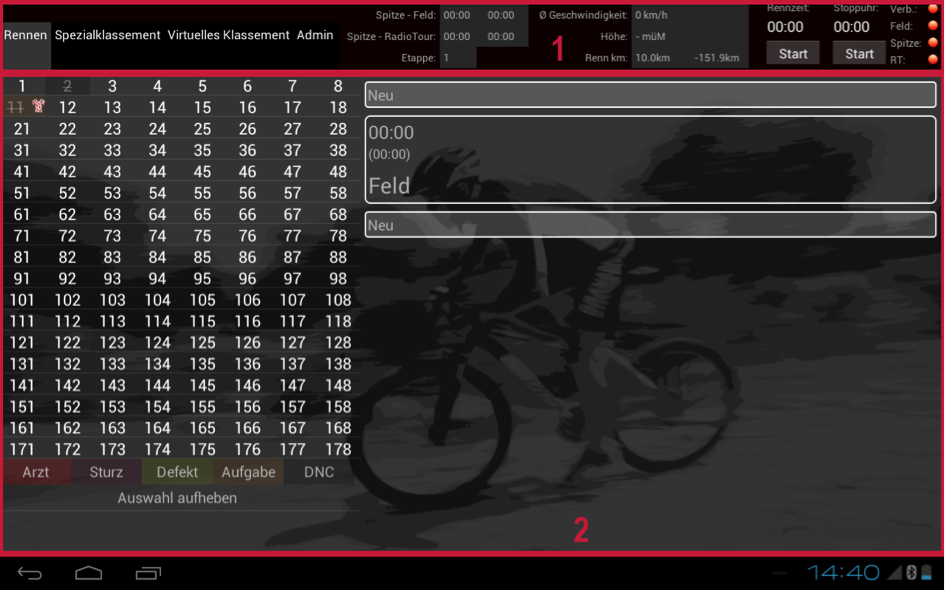
\includegraphics[scale=0.8]{07anhang/images/dev_activity.png}
\end{figure}

\subsection{Headerbereich}

\begin{figure}[h!]
\caption{Header Bereich}
\label{fig:headerbereich}
\centering
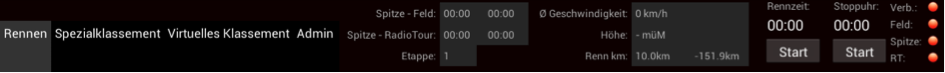
\includegraphics[scale=0.8]{07anhang/images/dev_header.png}
\end{figure}


\begin{lstlisting}{Name}
package ch.hsr.sa.radiotour.fragments;
public class HeaderFragment extends Fragment
	implements Observer, TimePickerIF
\end{lstlisting}

View definiert in:
\textit{res/layout/header\_fragment.xml}

Das \textit{HeaderFragment}, welches in Abbildung \ref{fig:headerbereich} illustriert ist, enthält alle Informationen, welche zu jedem Zeitpunkt der Applikationsausführung sichtbar sind. Dazu gehört der Systemzustand der zusätzlichen TourLive Komponenten welche via den TourLive Server über \gls{json} die \textit{RadioTour} Applikation mit Informationen versorgt.

Zudem werden wichtige Angaben zum derzeitigen Stand des Rennens im \textit{HeaderFragment} angezeigt, welche direkt aus der Tablet Anwendung stammen. Es sind dies die aktuelle Rennzeit und der aktuelle Rennkilometer, welcher, wie auch die aktuelle Höhe über Meer und die durchschnittliche Geschwindigkeit, aus dem im Tablet integrierten GPS Empfänger stammen. Um Fehlangaben zu korrigieren, ist die Kilometer- sowie die Rennzeitangabe editierbar.
Zeitabstände werden mit der ebenfalls im \textit{HeaderFragment} vorhandenen Stoppuhr gemessen. 
Mit einem Klick auf den "`Etappe"' Text wird die Marschtabelle, welche bereits absolvierte Stationen ausgraut, angezeigt.

\subsection{Hauptbereich}
Der Hauptbereich wird je nach ausgewähltem Tab (im Headerbereich) mit einem anderen Fragment ausgefüllt.
\\

\begin{figure}[h!]
\caption{RaceFragment}
\label{fig:racefragment}
\centering
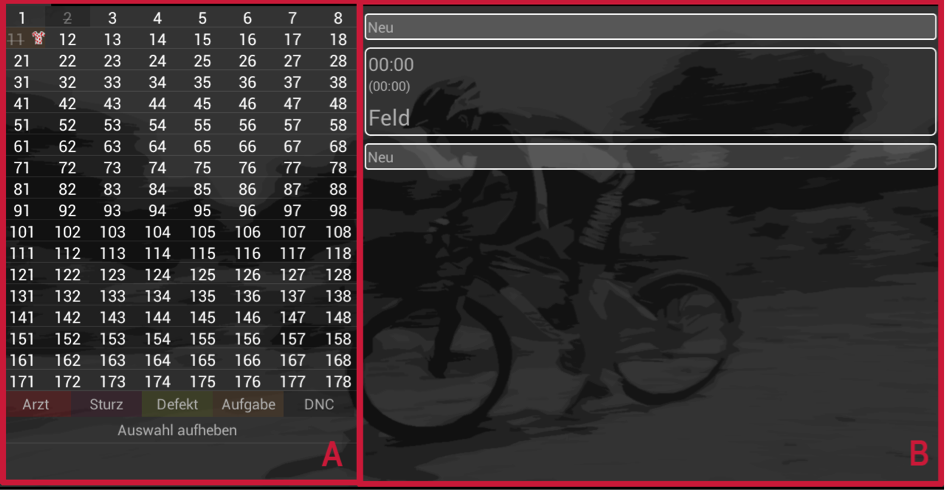
\includegraphics[scale=0.8]{07anhang/images/dev_racefragment.png}
\end{figure}


\textbf{RaceFragment.java}
\begin{lstlisting}{Name}
package ch.hsr.sa.radiotour.fragments;
public class RaceFragment extends Fragment 
\end{lstlisting}


View definiert in:
\textit{res/layout/race\_layout.xml}
\\
Das \textit{RaceFragment} welches in Abbildung \ref{fig:racefragment} zu sehen ist, beinhaltet zwei weitere Fragments. Das \textit{RaceFragment} an sich beinhaltet keine Funktionalität und dient nur zum Zusammenführen der zwei Fragmente \textit{DriverPickerFragment} und \textit{RiderGroupFragment}

\textbf{RiderPickerFragment}
\begin{lstlisting}{Name}
package ch.hsr.sa.radiotour.fragments;

public class RiderPickerFragment extends ListFragment
	implements OnClickListener
\end{lstlisting}

Das \textit{RiderPickerFragment}, Fragment A in Abbildung \ref{fig:racefragment} ermöglicht die Auswahl von einem oder mehreren Fahrern für die Zuweisung in eine Gruppe oder einem Spezialevent, siehe Abschnitt \ref{sec:requirements}. Die ausgewählten Fahrer können entweder per Drag and Drop oder mit anklicken des Zielfeldes zugewiesen werden. Mit einem Klick auf den "`Auswahl aufheben"' Text werden die bereits ausgewählten Fahrer wieder deselektiert.

Die Darstellung der Daten wird mithilfe eines \textit{ArrayAdapter<Team>} erzeugt. Dabei wird für jedes Team Objekt eine Zeile mit den jeweiligen Fahrern generiert. Die Textfelder mit den Spezialevents werden über eine dem \textit{RiderPickerFragment} hinzugefügten \textit{FooterView} ergänzt.

\textbf{RiderGroupFragment}
\begin{lstlisting}{Name}
package ch.hsr.sa.radiotour.fragments;

public class RiderPickerFragment extends Fragment
\end{lstlisting}


View definiert in:
\textit{res/layout/group\_fragment.xml}

Das \textit{RiderGroupFragment}, Fragment B in Abbildung \ref{fig:racefragment} stellt die aktuelle Rennsituation dar. Die schmaleren grauen Feldern dienen dazu, neue Gruppen zu erstellen. Wenn im \textit{RiderPickerFragment} Fahrer ausgewählt sind, können diese in die graue Fläche gezogen werden (Drag and Drop) oder auf die Fläche geklickt werden.
Den im transparenten Feld gruppierten Fahrer kann ein Rückstand relativ zur Spitze eingetragen werden. Dieser Rückstand wird den Fahrern welche dieser Gruppe angehören berechnet und im virtuellen Klassement berücksichtigt.
\\

\textbf{SpecialRankingFragment}
\begin{figure}[h!]
\caption{SpecialRankingFragment}
\label{fig:specialrankingfragment}
\centering
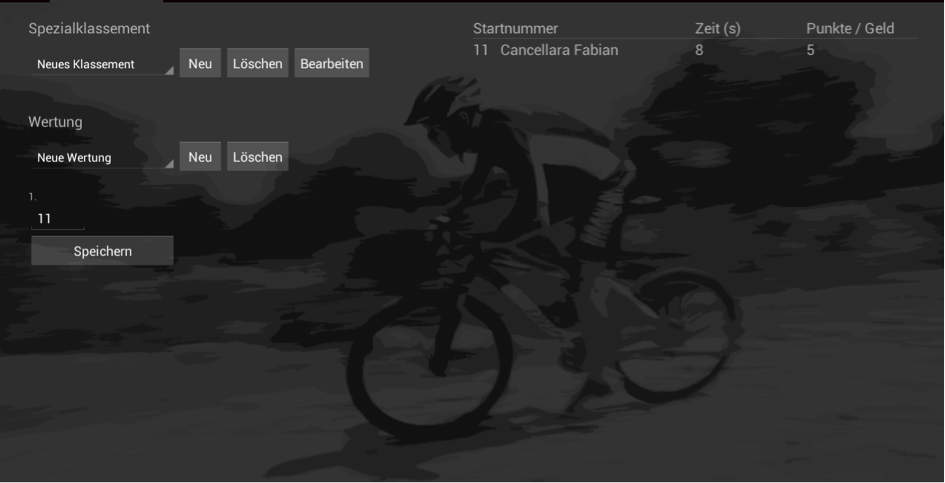
\includegraphics[scale=0.8]{07anhang/images/dev_specialranking.png}
\end{figure}


\begin{lstlisting}{Name}
package ch.hsr.sa.radiotour.fragments;

public class SpecialRankingFragment extends Fragment
\end{lstlisting}

View definiert in:
\textit{res/layout/special\_ranking\_fragment.xml}

Das \textit{SpecialRankingFragment}, abgebildet in Abbildung \ref{fig:specialrankingfragment}, erlaubt es neue Spezialklassemente und deren Wertungen, welche einer Etappe zugeordnet werden, zu erstellen. Eine Wertung beinhaltet Zeit- und/oder Punktebonus. Zudem kann jede Wertung eine unterschiedliche Anzahl berücksichtigte Anzahl Fahrer haben. Die Boni, welche Fahrer die in einer Wertung eine Klassierung erreichen, werden pro Spezialklassement rechts im \textit{SpecialRankingFragment} angezeigt. Die Etappenbasierte Verrechnung der Boni geschieht im \textit{VirtualRankingFragment}.




\textbf{VirtualRankingFragment}

\begin{figure}[h!]
\caption{VirtualRanking Fragment}
\label{fig:virtualrankingfragment}
\centering
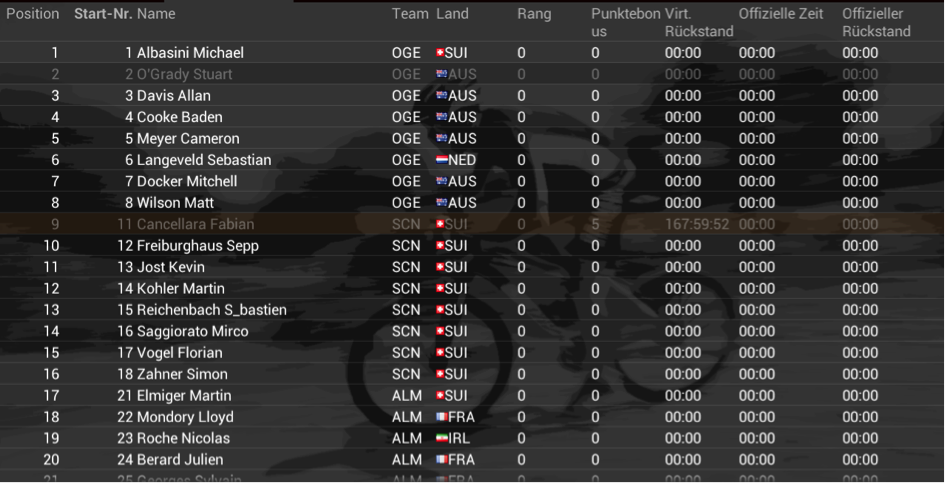
\includegraphics[scale=0.8]{07anhang/images/dev_virtual.png}
\end{figure}

\begin{lstlisting}{Name}
package ch.hsr.sa.radiotour.fragments;

public class VirtualRankingFragment extends ListFragment
\end{lstlisting}

Das \textit{VirtualRankingFragment} erbt von ListFragment und zeigt die zu der aktuell ausgewählten Etappe die dazugehörigen \textit{RiderStageConnection} (siehe Abbildung \ref{fig:domain}) an. Mit einem Klick auf einen Fahrer in der Rangliste lassen die Stammdaten des jeweiligen Fahrers verändern. So können zum Beispiel versehentlich als ausgeschieden markierte Fahrer wieder als im Rennen gesetzt werden. Über Klicks auf die  Spaltenbezeichnung lässt sich die Liste, sowohl auf- wie auch absteigend, nach den einzelnen Werten sortieren. Die Bezeichnung der aktuell sortierten Spalte wird fett dargestellt. Die Sortierung basiert auf der abstrakten \textit{RiderSortStrategy} Klasse, welche nach dem Vorbild des \textit{Strategy Pattern} implementiert wurde. 

\textbf{AdminFragment}

\begin{figure}[h!]
\caption{AdminFragment}
\label{fig:adminfragment}
\centering
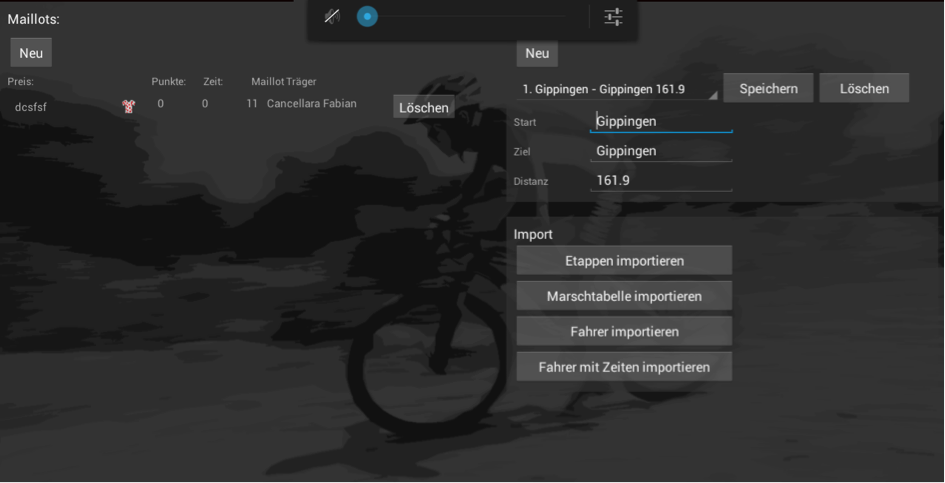
\includegraphics[scale=0.8]{07anhang/images/dev_adminfragment.png}
\end{figure}
\begin{lstlisting}{Name}
package ch.hsr.sa.radiotour.fragments;

public class AdminFragment extends Fragment
\end{lstlisting}


View definiert in:
\textit{res/layout/admin\_fragment.xml} 

Das \textit{AdminFragment}, Abbildung \ref{fig:adminfragment}, beinhaltet drei Grundfunktionen der Applikation.
Zum einen ist dies die gesamte Maillotsverwaltung inklusive Zuweisung eines Maillots zu einem Fahrer, der in der aktuellen Etappe dieses Maillot trägt.
Weiter wird im \textit{AdminFragment} die aktuelle Etappe ausgewählt. Zudem können neue Etappen erfasst oder bereits bestehende Etappen bearbeitet werden. 
Als letzte der drei Grundfunktionen steht der Import über csv zur Verfügung. Über einen Dateibrowser welcher in die Applikation integriert ist können die .csv - Dateien ausgewählt und importiert werden.  

\section{Kommunikation zum Server}



\section{Datenbankan}
\textbf{ORMLite (Version 4.39)}

 
Zur Speicherung der Objekte in die SQLite Datenbank des Tablet wird die Java Library ORMLite der Version 4.39 benutzt. In der Zwischenzeit sind neue Releases der Library auf der Webseite \url{http://ormlite.com/releases/} erschienen. Um sich in die Library einzulesen wird auf \url{http://ormlite.com/sqlite_java_android_orm.shtml} verwiesen.
\\
Um eine Änderung an den zu persistierenden Objekten durchzuführen ist es notwendig, die Klasse DatabaseConfigUtil.java im

\begin{lstlisting}{Name}
package ch.hsr.sa.radiotour.technicalservices.database;
\end{lstlisting}

als normale Java Applikation auszuführen. Dies generiert das \textit{Configuration File}

\textit{res/raw/ormlite\_config.txt}

welches für eine effizientere Ausführung von \textit{ORMLite} gebraucht wird.



